%
% Thesis template conforming to Williams College rules.
% Thanks to Ben Wood '08 and other contributors.
%

\documentclass[twoside]{report}
\usepackage[top=1.0in, bottom=1in, left=1.5in, right=1in, includehead]{geometry}
\pagestyle{headings}

\usepackage{setspace}

%% Special math fonts and symbols
\usepackage{amssymb}
\usepackage{amsfonts}
\usepackage{amsmath}
\usepackage{amsthm}
%% Rotate tables and figures
\usepackage{rotating}
%% Used for TODO items
\usepackage{color}
%% used for code listings.
\usepackage{float}
%% Used to replace LaTeX's ugly emptyset with diameter, which looks nicer.
\usepackage{wasysym}
%% Nicely formatted algorithms.
\usepackage{algorithmicx}
\usepackage[chapter]{algorithm}
\usepackage{algpseudocode}
%% Nicely formatted listings.
\usepackage{listings}
%% More kinds of arrow with stuff
\usepackage{empheq}
\usepackage{multicol}
\usepackage{subfigure}
%% Used for citations
\usepackage{cite}

%% Tell Latex to look in the `img` folder for images.
\graphicspath{ {images/} }

%%%%%%%%%%%%%%%%%%%%%%%%%%%%%
%% Thesis body %%
%%%%%%%%%%%%%%%%%%%%%%%%%%%%%

\begin{document}

%%%%%%%%%%%%%%%%%%%%%%%%%%%%%
%% Title page %%
%%%%%%%%%%%%%%%%%%%%%%%%%%%%%
\begin{titlepage}
  $\;$
  \vskip1.5in
  \onehalfspacing
  \begin{center}
    {\LARGE
      Predictive Pod Autoscaling in the Kubernetes Container Cluster Manager
    }
    \large
    \vskip.25in
    by\\
    Matt McNaughton\\
    \vskip.125in
    Professor Jeannie Albrecht, Advisor\\
    \singlespacing
    \vskip.5in
    \small
    A thesis submitted in partial fulfillment\\
    of the requirements for the\\
    Degree of Bachelor of Arts with Honors\\
    in Computer Science\\
    \vskip.5in
    Williams College\\
    Williamstown, Massachusetts\\
    \vskip.5in
    \today
    \vskip.5in
    {\Huge \textbf{DRAFT}}
  \end{center}
\end{titlepage}
%%%%%%%%%%%%%%%%%%%%%%%%%%%%%

\tableofcontents
% \listoffigures
% \listoftables

\onehalfspacing

\chapter*{Abstract}

\chapter*{Acknowledgments}

%%%%%%%% Chapters %%%%%%%%%%%%

%%%%% Introduction

\chapter{Introduction}

Over the past few decades, an explosion in the need for computing resources,
and the existence of cheap, interconnected computers, has
driven a significant increase in the feasibility and benefits of distributed
systems.\cite[pg. 1]{distributed-systems-principles-and-paradigms}

First, we consider the origin of distributed systems as a field of computer
science. Before the availability of cheap, powerful microprocessors and reliable,
efficient local-area networks (LANs), computational tasks could only be
performed on a singular computer.\cite[pg.
1]{distributed-systems-principles-and-paradigms} If a task was too
computationally expensive for a commodity PC, the only solution was to run
it on a larger, more powerful supercomputer. However, as cheap microprocessors
increased computers' availability, and LANs fostered quick inter-computer
communication, a new
model of performing resource intensive computation, distributed
systems, arose. In the distributed systems model, a collection of individual
computers function as a single computer to solve a given computational task.\cite[pg.
2]{distributed-systems-principles-and-paradigms}

Second, we consider the ever-growing interest in unlocking and implementing the
benefits of distributed systems. A number of forces drove, and continue to drive,
increased interest in distributed systems over
the past decade. The first, and most obvious, factor is the Internet.
As more people connected to the Internet, through computers,
mobile phones, and tablets, an increasing number of human interactions became
computerized. Consumption, communication, research, and more all
became possible on the Internet. Naturally, large amounts of computing resources
were needed to store the data, and perform the computational tasks, related to these
interactions. Closely coupled with this trend is the rise of ``Big Data''.
In 2013, the digital universe contained 4.4 zettabytes of data.\footnote{A
  zettabyte equals $10^{21}$ bytes, which equals 1 billion
terabytes.}\cite{the-digital-universe-of-opportunities} Naturally, without
multiple computers working together it would be impossible to store and process
this incredible volume of data. Today, it is nearly impossible to do
anything in modern society without interacting with a distributed system and
creating new digital data. Driving a car, trading a stock, visiting a doctor,
checking an email, and even playing a simple video game, are all activities that
distributed systems facilitate and improve.\cite[pg.
4]{distributed-systems-concepts-and-design} As life becomes more
computerized, and as the volume of data humans generate and hope to process
grows, distributed systems will only increase in importance.
Furthermore, research into distributed systems makes it possible to
continue to unlock, and make available to the general public,
the incredible power of networked, cooperating computers. As the distributed systems
supplying massive computational power become more
accessible, both because of decreased cost and increased ease of use and
reliability, we can
computationally address an ever increasing number of challenging, important problems.

There are a number of different models for computing tasks requiring high levels
of computing resources, including supercomputing, cluster computing, and grid
computing. In this thesis, we focus on cluster computing. Cluster computing
groups together similar commodity PCs on the same LAN to offer a singular mass
of computing resources. Specifically, we focus on the
cluster manager, an integral component of cluster computing. Cluster managers
are responsible for abstracting all of the management details of the distinct
nodes in the cluster, and instead presenting a single mass of computing resources
on which the user can run jobs or applications. In other words,
a cluster manager ``admits, schedules, starts, restarts, and monitors the full
range of applications'' on the cluster.\cite[pg. 1]{borg} There are a
variety of different cluster managers, the most important of which will be
discussed in the background chapter, each pursuing different objectives. This
thesis will ultimately focus on Kubernetes, an open-source cluster
manager from Google.\cite{k8s-website}

Cluster managers seek to accomplish a number of different goals, and as a
result, multiple metrics indicate success. For example, Microsoft's Autopilot is
predominantly concerned with application uptime, and thus success is measured
with respect to reliability and downtime.\cite[pg. 1]{autopilot}
Alternatively, a number of cluster managers measure themselves based on
efficient resource utilization (ERU).\cite[pg. 7]{borg} Essentially, efficient
resource utilization relates to the percent of cluster resources which are
actually being used. One such measurement of this goal, cluster
compaction, examines how many computers could be removed from the cluster, while
still comfortably running the cluster's current application load.\cite[pg.
5]{evaluating-job-packing-in-warehouse-scale-computing} This metric is
particularly important, because the more efficient the cluster management is at
utilizing resources, the less clusters cost, and the more accessible cluster
computing becomes to the general public. A final important
cluster management metric is quality of service (QOS). Quality of service measures the
ability of an application to function at a specified
performance level, despite ever-changing
external factors. Again, this metric is particularly important because
increasing the robustness of applications run on cluster managers means
these applications can be trusted with increasingly important tasks. Cluster
managers predominantly differ with respect to which metrics they optimize
for, and the process by which this optimization occurs.

\section{Goals}

This thesis is most concerned with maximizing the efficient resource utilization
(ERU) and quality of service (QOS) metrics with respect to the Kubernetes cluster manager.
As such, this thesis pursues three goals:

\begin{enumerate}
  \item Given an application running on a Kubernetes cluster, we seek to
    determine a method which ensures quality of
    service stays consistently high regardless of external factors. While it is
    difficult to make guarantees regarding quality of service, because
    application performance is dependent on a number of uncontrollable, varying
    external factors, it is possible to
    ensure each application has, and is utilizing, the resources it needs to
    function property. Given the cluster manager grants the application the
    resources it needs to function given the current external load,
    the cluster manager has done all it can to ensure a high quality of service.
  \item A simplistic solution to the first goal of ensuring a high application
    quality of service is to just give each application many more resources than
    it requests. Yet, this overallocation is inefficient and costly. Thus, our
    methods for ensuring a high quality of service must also ensure the
    maintenance, or improvement, of the efficient resource utilization metric.
    Thus, we add an additional goal: given a certain number of applications
    running on a Kubernetes cluster,
    we seek to determine a method which ensures the cluster is
    as small as possible, while still comfortably
    supporting the application's current, and future, resource needs.
  \item Given Kubernetes is an open-source project, we seek to implement, test, and
    evaluate a proposed enactment of the previous two goals.
    Thus, the methods we pursue will
    in part be dictated by the current structure and implementation of
    Kubernetes. Tests will be conducted using the Google Compute
    Engine\cite{google-compute-engine} on both
    simulated and real Kubernetes user data. The eventual goal is for this
    thesis' improvements to be merged into the production version of Kubernetes
    used to run 1000s of applications at Google everyday.
\end{enumerate}

\section{Contributions}

This thesis presents our given contributions to Kubernetes. Kubernetes seeks to
ensure high application quality of service and efficient resource utilization,
and our contributions look to further its ability to accomplish these
goals. As such, we present not only new methodology, but also new, working
implementations with the accompanying evaluation. We demonstrate the effectiveness
of our modifications in comparison to the non-modified Kubernetes using both
simulated and real-world datasets. Finally, we
discuss the experiences of making these modifications to Kubernetes, as well as
avenues for future improvements with respect to Kubernetes and cluster managers in
general.

\section{Contents}

@TODO - This section can not be written until the thesis is completed.

\chapter{Background}

\section{Resource Intensive Computing Paradigms}

As was briefly mentioned in the introduction, a number of different paradigms
exist for undertaking computing tasks too resource intensive for a single
computer. They are discussed in detail below:

\begin{enumerate}
  \item \underline{Supercomputing}: The supercomputing model responds to
    increased demands for computing resources by increasing the technical
    specifications of the computer far beyond the range of the
    traditional commodity PC.
    While supercomputers are able to avoid the majority of the complications
    resulting from the introduction of networks, most prominently reliability and
    security, there are naturally limits on the power of supercomputers.
    Importantly, constructing supercomputers is extremely expensive, and thus
    their computing power is not available to the general public. Furthermore,
    it is difficult to scale a supercomputer should the need arise. Finally,
    supercomputers offer a single point of failure, meaning they are not
    particularly robust to error. These limitations have decreased the usage of
    supercomputers to provide the mass of computing power needed in the ``Big
    Data'' era.

  \item \underline{Cluster Computing}: Cluster computing is defined as utilizing
    ``a collection of similar workstations of PCs, losely connected by means of
    a high-speed local-area network [where] each node runs the same operating
    system.''\cite[pg. 17-18]{distributed-systems-principles-and-paradigms}
    Cluster computing can provide a mass of computing power similar to
    that contained in a supercomputer. Cluster computing also offers many
    advantages over the single supercomputer. First, and perhaps most
    importantly, they are much more cost-efficient, and thus much more
    accessible. Second, clusters are easy to
    scale by simply adding new commodity PCs as nodes.
    Finally, cluster computing is much more fault
    tolerant, as a single failing commodity computer will simply be removed
    from the cluster. Cluster computing is used in the
    implementation of what is colloquially referred to as \textit{Cloud
    computing}, in which large amounts of computing resources are offered on a
    per-usage basis.\cite[pg. 13]{distributed-systems-concepts-and-design}
    Cloud computing, as implemented by Amazon Web
    Services,\cite{amazon-web-services} Microsoft Azure,\cite{microsoft-azure}
    and Google Compute Engine,\cite{google-compute-engine} continue to
    revolutionize the development and deployment of computing applications, as
    developers gain access to cheap, easily accessible, and quickly scalable
    computing power.

    \begin{figure}[!h]
      \centerline{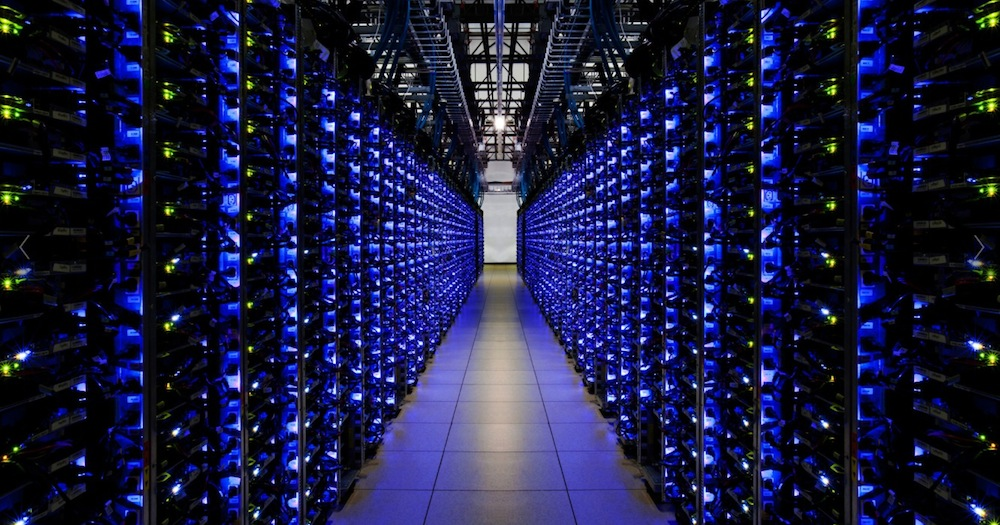
\includegraphics[scale=.4]{google-cluster.jpg}}
      \caption{A Google Computing Cluster.\cite{image-google-cluster}}
    \end{figure}

  \item \underline{Grid Computing}: Grid computing is similar to concept in
    cluster computing, except it foregoes the requirement that all computers
    within the grid be relatively homogeneous. As such, the grid computing model accounts
    for a large degree of heterogeneity with respect to network membership,
    operating system, hardware, and more.\cite[pg.
    18]{distributed-systems-principles-and-paradigms} While grid computing
    systems lack of homogeneity requirements increase flexibility,
    the resulting heterogeneity introduces significant complexity.

\end{enumerate}

Ultimately, because of simplicity, cost, and scalability, cluster computing is
the most prominent resource intensive computing paradigm. Thus, cluster
computing, and the accompanying cluster manager, is the focus of this
thesis.

\section{Cluster Management Paradigms}

As was briefly mentioned in the introduction, cluster managers are responsible
for admitting, scheduling, running, maintaining, and monitoring all applications
and jobs a user wishes to run on the cluster. Naturally, cluster managers are
extremely diverse, both in the types of applications and jobs they are most
suited to running, and the method in which they seek execute their duties.
At the most basic level, there are two types of workload that may be submitted
to a cluster manager: production and batch. Production tasks are long-running
with strict performance requirements and penalties to downtime. Batch tasks are
more flexible in their ability to handle short-term performance variance. In the
context of a large company like Google, a production task would be serving a
large website like Gmail, which must be continuously accessible with low-latency
and little downtime. A batch task would be analysing advertising analytics data
with MapReduce, which can fail or slow without significant external
costs.\cite[pg. 1]{borg} The type of tasks a cluster management system
predominantly seeks to run dictate the cluster manager's implementation details.

One important decision in the implementation of a cluster manager is the manner
by which the cluster manager schedules jobs.\footnote{Scheduling jobs on
machines simply equates to assigning jobs to resources on a machine.}  There exist three
different methods of scheduling: monolithic, two-level, and
shared state. With monolithic scheduling, a single algorithm
is responsible for taking the resource requests of all jobs and assigning them
to the proper machine. With two-level scheduling, the cluster manager simply
offers resources, which can then be accepted or rejected by the distributed
computing frameworks.\footnote{Distributed computing frameworks are frameworks
built to function over multiple machines: Apache Hadoop, Apache Spark\dots}
Finally, with shared state scheduling, multiple different algorithms concurrently work to
schedule jobs on the cluster.\cite[pg. 1]{omega} Naturally, all
of these methods have positives and negatives. While monolithic scheduling is
simple to initially, a single-threaded monolithic scheduler does not allow
nuanced processing of jobs. Attempts to add this nuance can create an incredibly
complicated algorithm that is difficult to extend.\cite[pg. 353-354]{omega}
While two-level scheduling is lightweight, simple, and offers advantages with respect to
data locality, it is not effective for long-running,
production jobs. Finally, while shared state scheduling removes the scheduler as
both a computational and complexity bottleneck, yet must take steps to guarantee
global properties of the cluster.\cite[pg. 363]{omega}
The ultimate determined method of assigning a job
resources effects the type of applications and distributed computing frameworks
runnable on the cluster manager and the efficiency with which these applications
and frameworks run.

A final distinction is licensing and availability of the cluster manager's code.
Because entities need cluster managers only to process and store massive amounts
of data and human-computer interaction, mainly large
corporations develop and utilize cluster managers. Often these cluster
managers are kept within the confines of the corporation, or only explained by a
brief paper or conference talk, with little source code available. In more
unique cases, the company will open-source the source code, allowing anyone to
view, modify, and run the cluster manager. Such open-sourcing presents a unique opportunity
for researchers wishing to experiment with cluster managers, yet without the
resources to create their own from scratch. In rarer instances, a
fully-developed cluster manager will originate from academic research. In unique
scenarios, a large corporation will use this cluster manager and the full code will
be open-sourced. The availability of source code directly impacts the
feasibility of pursuing experiments with an already existing cluster management
system.

Naturally, cluster managers can vary in multiple additional ways. However,
the previous three differences recognize the most important distinctions in this
thesis' context. Given this understanding, we can know begin to examine specific
cluster management implementations and defend our choice of Kubernetes as the
cluster manager on which we will ask and answer our research question.

\subsection{Borg}

While just recently described to the public in a 2015 paper, the
\textit{Borg} cluster manager from Google has been in use for over a
decade.\cite[pg. 14]{borg} Borg incorporates
many different objectives, seeking to abstract resource management and failure
handling, maintain high availability, and efficiently utilize resources on the
cluster.\cite[pg. 1]{borg} It is responsible for managing the hundreds of
thousands of batch and production jobs run everyday at Google. Additionally,
Borg utilizes a monolithic scheduler, as jobs specify the
resources they need, and a single Borg scheduler decides whether to admit and
schedule said jobs. Finally, Borg is not open-source. In fact, it was not even
publicly announced or described until 2015, despite running at Google for over a
decade. However, Kubernetes, Google's open-source cluster manager, incoporates
much of the work done to implement and improve Borg.

\subsection{Omega}

Also originating at Google, \textit{Omega} is a cluster manager seen as the
current-day extension of Borg. While retaining the mission and goals of Borg,
Omega differs in implementation. Specifically, it considers a new method of
assigning jobs the resources they need on the cluster by implementing
shared state, instead of monolithic, scheduling. As mentioned in the general
overview, shared state scheduling allows multiple scheduling algorithms to work
in parallel to assign tasks the resources they request. Research on Omega shows
this parallel scheduling implementation both eases the complexity of adding new
scheduling behaviors and offers competitive scaling performance.\cite[pg.
358-359]{omega} Additionally, in Omega, all schedulers are aware of the entire
state of the cluster, meaning that the resource allocation to a job can be
varied after the job begins to execute. This flexibility offers significant
performance improvements.\cite[pg.352]{omega} Like Borg, Omega is not
open-source. However, like Borg, much of the work done on Omega is incorporated
into Kubernetes, Google's open-source cluster manager.

%%% Cluster manager table.

\begin{table}[]
\centering
\caption{Overview of Cluster Management Paradigms.}
\begin{tabular}{|l|l|l|l|}
\hline
                    & \textbf{Job Type} & \textbf{Scheduling Model} &
                    \textbf{Open Source} \\ \hline
\textbf{Borg}       & Both              & Monolithic                & No
\\ \hline
\textbf{Omega}      & Both              & Shared state              & No
\\ \hline
\textbf{Mesos}      & Batch             & Two-level                 & Yes
\\ \hline
\textbf{YARN}       & Batch             & Monolithic                & Yes
\\ \hline
\textbf{Kubernetes} & Production        & Monolithic                & Yes
\\ \hline
\end{tabular}
\end{table}

\subsection{Mesos}

Lest we think all cluster managers originate at Google, we now examine Apache
Mesos, a cluster manager originating at University of California, Berkeley, and
currently at use at a number of prominent corporations including Twitter. Mesos
is much more lightweight than either Borg or Omega, and simply seeks to offer
resources to distributed computing frameworks (i.e. Apache Hadoop, Apache
Spark\dots) which can decide to accept or reject these resources. It does not
seek to monitor the health of jobs or provide user-interfaces for viewing the
current state of a job, leaving those tasks to the distributed computing
framework. Additionally, Mesos predominantly focuses on quick-running,
high-volume batch jobs, and is not particularly suited to long-running,
high-availability production jobs.\cite[pg. 358]{omega} In part, Mesos'
job scheduling implementation specifics the singularity of the job types
Mesos efficiently processes. Mesos utilizes two-level scheduling, in which the
cluster management system simply offers, not assigns, available
resources to the distributed computing framework. Predominantly, this decision
is made to ensure data locality.\cite[pg. 1]{mesos} Data locality is a measure
of if the task has the necessary data on its machine, or if it must make a
costly request across the network for the data. Mesos works to ensure data
locality by allowing multiple frameworks to function on the same machines, and
thus share data, and also for frameworks to dictate their own resources, such
that they can work to ensure data locality. If running a large number of data
processing tasks, with extremely high volumes of data, data locality can be
essential to efficient cluster operation. Finally, Mesos is interesting in
that it is entirely open-source, yet still in use at some of the largest tech
companies.

\subsection{YARN}

We now briefly discuss Apache Hadoop YARN. YARN, an acronym for \textit{Yet Another
Resource Negotiator}, is a cluster manager initially built for use with Apache
Hadoop.\cite[pg. 1]{yarn} However, it is now possible to use YARN with a variety
of distributed computing frameworks. Unsurprisingly given YARN's initial use
case, YARN is predominantly used for running batch jobs.\footnote{At the time of
the publication, YARN was just beginning to be used for production jobs;
however, its main focus from creation has been batch processing.\cite[pg.
11]{yarn}} Like Mesos, YARN aims to support data-locality,
again a predominant advantage for batch processing.\cite[pg. 3]{yarn} YARN
schedules resources by allowing per distributed computing framework application
masters to request resources from a single resource master.\cite[pg. 5]{yarn} As
a single resource master is assigning all of these resources, YARN is a
monolithic scheduler. Similar to Mesos, YARN is both entirely open-source and in use
at major corporations like Yahoo.\cite[pg. 9]{yarn}

\subsection{Kubernetes}

Finally, we arrive at the cluster management that is the focus of this thesis:
Kubernetes. Kubernetes also originates, although it is open source, meaning
anyone is free to modify and deploy Kubernetes. Kubernetes is also the most
recent of the cluster managers we consider in this background research
section.\footnote{Kubernetes became public in the summer of 2014.} The recent
explosion in popularity of containerization\footnote{We discuss both the motivations and
technology behind containerization in the Appendix. Briefly, containerization is
packing everything an application needs to run into a single \textit{container}
and then running that container on any desired computer.}
heavily impacts the development and implementation of Kubernetes. Specifically,
Kubernetes is seen as part of a new paradigm of developing applications
through the use of microservices.\footnote{Again, we will
discuss microservices in greater detail
in the Appendix. Essentially, microservices are the division of applications
into small, easily scalable services which communicate with each other across
the network.} Kubernetes predominantly focuses on effectively running service
jobs. As previously mentioned, these jobs require
high-availability and potentially varying amounts of resources. Additionally,
Kubernetes currently utilizes a monolithic, fairly simple scheduler, although
there are plans to grow the scheduler in the future.\cite{k8s-design-overview}
Finally, Kubernetes is an open source project, yet is also used in production at
Google, and available to the public through the Google Container
Engine.\cite{google-container-engine}

We choose Kubernetes as the cluster manager on which to conduct our experiments
for a number of reasons. First, Kubernetes focuses on service jobs. Services jobs
have particularly stringent requirements for availability and are also the most
likely to have varying resource needs. Both these conditions are closely linked
with the previously stated goals of this thesis, and Kubernetes is the cluster
manager that stands to benefit the most if we achieve our goals. Additionally,
Kubernetes is the only cluster manager focusing on long-running services that is
open source. Focusing on a open source cluster manager allows us to benefit from
the previous work of others, as well as expand the potential benefits of any
successful work.

\section{Auto-scaling Paradigms}

We now proceed to consider a subset of cluster management closely related to
this thesis' goal of ensuring high quality of service in the face of changing
external factors and efficient resource utilization. Specifically, we introduce
auto-scaling, a method of ensuring each application has the necessary amount
of resources to handle its varying load.\footnote{Importantly, auto-scaling is
made possible by current models of cluster\/cloud computing, in which it is
possible to automatically obtain and relinquish computing resources within a
very short time frame. Obviously, if adding computing resources required buying
a new physical server, as was the case before the advent of cloud computing,
auto-scaling becomes impossible.}

To better understand both the implementation and benefits of auto-scaling, let
us consider a simple scenario. Imagine you have an application running on a
cluster for a week. On Monday, it will need $x$ resources.\footnote{By
  \textit{resources}, we mean CPU, memory\dots} On Tuesday through
Thursday, the application will need $2x$ resources. Finally, on Friday the
application will again need $x$ resources. Without auto-scaling, we are forced
to assign a constant amount of resources to the application running on our
cluster. However, there is no constant amount of resources that can meet
the two goals of efficiently utilizing the cluster's resources and ensuring the
application has the resources it needs to maintain a high-level of service. If
we assign the application $x$ resources, then on Tuesday through Thursday the
application will not have the amount of resources it needs to handle its load,
and quality of service will deteriorate. Alternatively, if we assign the
application $2x$ resources on the cluster, than on Monday and Friday we will
essentially be wasting $x$ resources on the cluster, as they are assigned to an
application that does not need them. This waste prevents reaching our goal of
efficiently utilizing the cluster's resources.

We address the inability to find a static amount of resources efficiently
handling all the variances in application load through auto-scaling.
Auto-scaling allows us to assign an application more or less resources on the
cluster based on varying external factors. In our previous example, auto-scaling
would allow us to assign the cluster $x$ resources on Monday and Friday and
$2x$ resources on Tuesday through Thursday. Through auto-scaling, we accomplish
both goals: our application has the resources it needs to ensure a high quality
of service, and our application is not inefficiently holding cluster resources
that it does not need. Overall, Auto-scaling can make applications on a cluster more
cost-effective and more performant.

Given an understanding of the importance of auto-scaling, we now begin the
examine the differing implementations of auto-scaling. Auto-scaling
implementations differ in how they assign an application the new resources it
needs\footnote{Auto-scaling implementations can also take away resources from
an application running on a cluster.} and how they decide to
assign the application the resources it needs.
There are two predominant characteristics shaping the nature of an autoscaling
implementation. The first is if the auto-scaling is horizontal or vertical. The
second is if the auto-scaling is reactive or predictive.

We begin by examining the difference between horizontal and vertical scaling.
Let us begin by assuming there is an application running on a virtual machine
instance assigned by the cluster with $x$ amount of resources. The application
now faces external load such that the current amount of resources assigned to
the application is not sufficient. Rather, let us assume the application now
needs $2x$ resources to function efficiently. There are now two options. In
\textit{vertical} auto-scaling, the cluster manager will attempt to assign the
virtual machine instance running the application the needed $2x$ resources
without halting the execution of the application. In \textit{horizontal}
auto-scaling, the cluster manager will create another instance of the virtual
machine running the application, so that there are now two machines each with
$x$ resources ($2x$ resources in summation). The load will now be split between
the two new instances of the application, meaning each machine must only handle
requests requiring the $x$ resources each individual virtual machine instance
has.\cite[pg.
4]{auto-scaling-techniques-for-elastic-applications-in-cloud-environments} While
both of these variations of auto-scaling accomplish the same purpose, horizontal
auto-scaling is much simpler. Given we know how to create an instance of a
virtual machine running the application, which is an entirely safe assumption
considering we already created one such instance, it is fairly trivial to create
another instance, and then split the load between these two instances using
standard methods of load balancing. This
statement of simplicity of course assumes the application is written in a
scalable manner such that it can be replicated with no unexpected modifications
on operation. Contrast this well-defined with more questionable, difficult
process of changing the resources given to a virtual machine without stopping
the application from executing. Importantly, there exists
no consistent, cross-platform method of
modifying the amount of resources granted to a virtual machine instance without
stopping the execution of the virtual machine. As a result, every method of
auto-scaling we examine focuses on horizontal auto-scaling.\cite[pg.
4]{auto-scaling-techniques-for-elastic-applications-in-cloud-environments}

We continue by examining the distinction between reactive and predictive
auto-scaling. At the simplest level, \textit{reactive} auto-scaling reacts to
the current state of the application and cluster, while \textit{predictive}
auto-scaling predicts the current state of the application and cluster.\cite[pg.
12]{auto-scaling-techniques-for-elastic-applications-in-cloud-environments}
Predictive auto-scaling can be based on a number of different metrics and
methods of prediction, which highlights some of the inherent complexity of
predictive auto-scaling. While reactive auto-scaling must only consider one
method of gathering and interpreting information, when attempting predictive
auto-scaling there are many decisions that must be made with respect to the
most accurate method of projecting past metrics into future metrics. However,
predictive auto-scaling has the advantages both of incorporating greater amounts
of past information which may be able to provide historical insight and allowing
the cluster manager to decrease the time-costs of certain actions by performing
them before a reactive cluster manager would suggest.\footnote{We will spend
considerable time later in this concept. Basically, predictive auto-scaling
makes it easier to account for the amount of time necessary to perform
horizontal auto-scaling (i.e. creating a new virtual machine instance running
the application). If we know we need a machine in the future, we can start
creating it now, so it is ready by the time it is needed. With reactive
auto-scaling, we do not know we need the replication until the current state of
the application and cluster indicates it. Thus, we must wait for the
auto-scaling to occur, all the while the application will be operating with
sub-optimal resources.}
Finally, techniques for auto-scaling can be both reactive and predictive as
they incorporate both current and projected cluster and application information
to make auto-scaling decisions.

A number of the major providers of cloud computing resources offer auto-scaling.
The most prominent of these providers is Amazon, which supports threshold-based
horizontal auto-scaling on EC2 virtual machine
instances.\cite{amazon-auto-scaling-developer-guide} Furthermore, Netflix
implements time-series analysis auto-scaling to help it respond to the
varying demand placed on its services throughout the
day.\cite{netflix-scryer-part-i} Finally, Kubernetes
implements control-theory auto-scaling.\cite{k8s-horizontal-pod-autoscaler-proposal}
We will examine threshold, time-series analysis, and control-theory
auto-scaling in detail in the remainder of this section.

%% Auto-scaling Paradigms Table

\begin{table}[]
\centering
\caption{Overview of Auto-scaling Paradigms.}
\begin{tabular}{|l|l|l|}
\hline
                    & \textbf{Reactive vs Predictive} & \textbf{Implementors} \\ \hline
\textbf{Threshold}  & Reactive                        & Amazon Web Services   \\ \hline
\textbf{Time-Series Analysis} & Predictive            & Netflix               \\ \hline
\textbf{Control-Theory} & Both (currently reactive)   & Kubernetes            \\ \hline
\end{tabular}
\end{table}


\subsection{Threshold-based Rule Policies}

\subsection{Time-series Analysis}

\subsection{Control-Theory}

\subsubsection{Model Predictive Control}

\section{Summary}

\chapter{Appendix}

\section{Technologies Underlying Kubernetes}

\subsection{Containerization}

\subsubsection{Virtualization}

\subsubsection{Containerization}

\subsubsection{Docker}

\section{Trends Motivating Kubernetes}

\subsection{Microservices}

%%%%%%%% References %%%%%%%%%%
\bibliographystyle{acm}
\bibliography{thesis}
%%%%%%%% End References %%%%%%
\end{document}
